%%%%%%%%%%%%%%%%%%%%%%%%%%%%%%%%%%%%%%%%%%%%%%%%%%%%%%%%%%%%%%%%%%%%%%%%%%%%%%%%%%%%%
% Machine Learning in Monitoring
%
% 1. Anomaly detection
%  - Adaptive using classifier updates
% 2. Alarm management
%  - Adaptive using RL
% 
%%%%%%%%%%%%%%%%%%%%%%%%%%%%%%%%%%%%%%%%%%%%%%%%%%%%%%%%%%%%%%%%%%%%%%%%%%%%%%%%%%%

ML prediction applications are effective complements to existing infrastructure in the process industry through soft sensors, state estimation, and forecasting. However, they are limited in applications regarding safety and risk management.  In the process industry, safety is upheld as the greatest \textit{value}; investing in a successful safety system is just good business.  

\begin{quote}
    "Safety is a \textbf{value}, not a priority.  Priorities change, but company values never do." \\
    --- Rex Tillerson, ex-CEO of ExxonMobil
\end{quote}

Decades ago, process safety investments are frowned upon by management due to its high costs and \textit{invisible} returns. In fact, construction workers used to cheer when project supervisors announced that \textit{only} 20 deaths will incur for this project---an event completely unacceptable in today's standards. Indeed, a perfect safety and risk management system results in \textit{no change} in day-to-day activities because all the incidents are proactively mitigated. As such, it is incredibly easy to become complacent towards risk management. However, if safety takes a back seat, the occurrence of the next incident is not a matter of if, its a matter of \textit{when}. Therefore, safety must be proactively (not reactively) managed to safeguard people, the environment, company assets, and production capabilities in terms of physical equipment and the social license to operate. Here, ML can be leveraged to proactively monitor process systems and create an additional layer of safety. In this chapter, ML algorithms will be applied to detect and predict equipment failures, process abnormalities, process variability and also perform alarm management. Through these applications, ML will be used to create multi-variate alarm systems that explore multi-variable interaction effects and gives fewer false alarms. Additionally, a new alarm management system that specifically tackles alarm flood scenarios will be introduced.  The objectives of this system are twofold: 1) Reduce sheer number of alarms during a flooding scenario; 2) identify the most important alarms so operators can prioritize safety critical alarms.

This chapter is organized as follows: Section 1 introduces data pre-processing methods for anomaly detection/prediction applications where the data is heavily imbalanced.  Section 2 introduces the anomaly detection and prediction algorithms and section 3 concludes this chapter with an introduction to a novel approach for alarm management.

The main contributions of this chapter are the data pre-processing methods used to prepare data sets for anomaly detection/prediction.  Additionally, it was shown that using synthetic data was able to enhance accuracy.  Lastly, a novel alarm management approach based on reinforcement learning was introduced to filter nuisance alarms and sort alarms based on their priority.  


\section{Data Pre-processing for Monitoring}
Data containing anomalous and/or incident events are extremely rare---thankfully---in the process industry. \begin{quote}
    Anomaly or anomalous activity: An abnormal or unexpected event given other variables (often multivariate).  For example, a person walking in a t-shirt when it is -$\ang{30}$ C outside.
\end{quote}

In fact, it is not uncommon to have just one incident in a data set containing hundreds of thousands of records.  Under such circumstances, building ML models to identify incidents is extremely difficult.  Remember, ML models are nothing more than statistical models with training formulated in an incremental updating fashion. In the scenario where the training data set contains 999,999 non-anomalous activities with 1 anomalous activity, the model will simply learn to return non-anomalous for all inputs; such a model would still achieve 99.9999\% accuracy on the training data!  When a human is provided with this data set, the human would instead focus most of its attention on the one anomalous activity, studying how it is different from all the other points.  A \textit{tabula rasa} machine is simply not equipped with such cognitive abilities, and will treat every data point equally; however, humans can artificially provide cognition to the machine.

\subsection{Data Prep for Anomaly Detection}
Anomaly \textit{detection} tasks are quite simple compared to anomaly \textit{prediction} tasks that will be discussed later on in this section. In anomaly detection, the model simply has to classify if there is an anomaly at current time. For example, given some states of a reactor, is the output temperature anomalous? That is, is the measured output temperature expected given the states?  Of course, such questions are difficult for humans to answer, especially in multi-variate environments; however, such questions can easily be answered by machines. Unfortunately, the events that are of interest to us (anomalies) are, often times, significantly more rare compared to normal process data. Hence, the leading reason for poor model performance in imbalanced data sets (i.e., distribution of different classes are vastly different) is the \textit{imbalanced} nature.  There exists two traditional ways to tackle the data imbalance issue: \textbf{undersampling} and \textbf{oversampling} \cite{under_over_sampling}.  Objectively, both methods aim to re-balance the data set so that the positive and negative data are in harmony.

A visual description of undersampling and oversampling is shown in Figure \ref{fig:03under_over_sampling}. In undersampling, the majority class(es) are significantly down-sampled to be the same size as the minority class.  The obvious flaw with this technique is the significant data in-efficiency.  In this method, the majority of the data that may contain critical features and information are simply discarded.  To take advantage of the whole data set, oversampling is sometimes used.  In oversampling, the minority class data is copied $n$ times until is approximately equivalent to the majority class.  Although oversampling allows the whole data set to be used, the models built typically overfit to the minority data simply because it was copied so many times.  During deployment, anomalies that are even slightly different from the ones in the training minority data set are often times misclassified.

Another more mathematical way to tackle this data imbalance issue is to bias the cost function to \textbf{heavily} discourage misclassification of positive samples.  However, such a methods requires tuning of the cost function, and is often times difficult.

\begin{figure}[H]
    \centering
    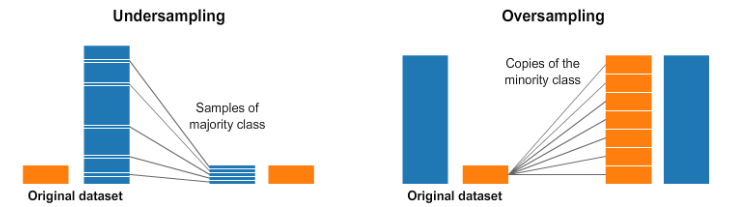
\includegraphics[width=0.8\textwidth]{images/ch3/over_and_undersampling.jpeg}
    \caption{A visual representation of undersampling (left) and oversampling (right). Original image from Kaggle.}
    \label{fig:03under_over_sampling}
\end{figure}

Luckily, normal process data are typically plentiful and lack "increasing" information (i.e., data is typically from steady state processes that hover around the same value for weeks) in the process industry.  Therefore, discarding large bulks of data in certain processes do not affect the ultimate accuracy of the model.  For anomaly detection, the majority class data was first undersampled to be comparable to the minority class. Undersampling should uniformly sample the data set to ensure all operating regimes are sufficiently captured. Then, a label column is generated; all anomalous events were given a value of 1 and normal process data had labels of 0.  An example of undersampling is shown below.  In this example, the process is deemed anomalous when $x_1 + x_2 > 3$.

\begin{table}[h]
    \centering
    \begin{tabular}{ c | c | c }
        $x_1$ & $x_2$ & label \\
        \hline
        2 & -1 & 0 \\
        3 & 0 & 0 \\
        2 & 5 & 1 \\
        2 & -2 & 0 \\
        5 & -1 & 1 \\
        -2 & -1 & 0 \\
        1 & -3 & 0 \\
        2 & -4 & 0 \\
        -2 & 2 & 0 \\
        -2 & 4 & 0 \\
    \end{tabular}
    \caption{Original data set before undersampling.}
    \label{tab:03undersampling}
\end{table}

Notice that in Table \ref{tab:03undersampling}, the majority class dominates the minority class 5:1.  After downsampling, the data set becomes:

\begin{table}[h]
    \centering
    \begin{tabular}{ c | c | c }
        $x_1$ & $x_2$ & label \\
        \hline
        2 & 5 & 1 \\
        2 & -2 & 0 \\
        5 & -1 & 1 \\
        -2 & -1 & 0 \\
    \end{tabular}
    \caption{Original data set before undersampling.}
    \label{tab:03undersampling2}
\end{table}
Note that the majority and minority class do not have to be perfectly balanced, especially in cases where perfectly balancing the classes require discarding unique information from the majority class.

\subsection{Data Prep. for Anomaly Prediction}
Anomaly prediction is a much more difficult problem compared to anomaly detection.  In anomaly prediction, the model must \textit{predict} if an anomaly is going to happen \textit{before} it happens.  Compared to anomaly detection, this task is much more difficult, and how far in advance an anomaly can be detected is heavily dependent on the speed of dynamics of the system.  For example, in cat classification, anomaly detection simply has to identify if the picture is a cat or not.  However, anomaly prediction has to predict if the animal in each picture will eventually grow up to become a cat.

In anomaly prediction, the data is first labelled as in anomaly detection. Afterwards, the data is augmented as follows:
\begin{equation}
    x = [x_{t - l - L}, ...,  x_{t - l - 3}, x_{t - l - 2},  x_{t - l - 1},  x_{t - l}]
    \label{eq:03prediction}
\end{equation}
where $l > 0$ denotes the minimum number of sampling time the model should predict in advance.  $L$ represents the amount of previous information to be provided to the model. Note that even though an $l$ of 10 is chosen, this does not guarantee that the model will always predict anomalies 10 time steps in advance. Moreover, if the model predicts positive, it does not mean that an anomaly will occur exactly 10 time steps later. Merely, it just biases the algorithm to be more effective around that time range. How early an anomaly can be detected is purely dependent upon the dynamics of the system.  For example, if the degradation of an equipment is slow and gradual, the anomaly might be detected days in advance; however, an instantaneous failure offers no time for any early detection.

Like in anomaly detection, the data is heavily skewed towards normal process data; therefore, the majority class must also be downsampled to be comparable to the minority data set. Downsampling occurs last to ensure no temporal relationships are broken. A quantitative example for the augmentation of an anomalous data is shown below.  Here, suppose downsampling is not required (since an example is already shown above) and $l = 1; L = 2$.

\begin{table}[h]
    \centering
    \begin{tabular}{ c | c | c }
        $time$ & $x_2$ & label \\
        \hline
        0 & 5 & 0 \\
        1 & 3 & 0 \\
        2 & 7 & 0 \\
        3 & 6 & 0 \\
        4 & 4 & 0 \\
        5 & 2 & 0 \\
        6 & -1 & 1 \\
        7 & -3 & 0 \\
        8 & -1 & 0 \\
        9 & 2 & 0 \\
    \end{tabular}
    \caption{An arbitrary time-series data set.}
    \label{tab:03aug}
\end{table}

From Table \ref{tab:03aug}, the time series augmented data point for the anomalous event would be:
$$x = [x_3, x_4, x_5]$$
$$x = [6, 4, 2]$$


\subsection{Synthetic Data Generation}
In the above methods, the assumption of plentiful data was made.  In industry, this is not always true, especially for the anomalous data.  Here, three different \textit{synthetic} data generation methods will be introduced, with each method generating fake, yet similar, minority class data.  This topic is an especially popular research topic for the computer vision field where good, labeled data are rare. In fact, many "Completely Automated Public Turing test to tell Computers and Humans Apart" (CAPTCHAs) use traffic signs to force potential users of the website to first label some data, before being allowed to proceed. Most likely, the labeled data are then sold to computer vision companies. The main idea of synthetic data generation is to construct fake data that is \textit{exactly equivalent} to the real data that even a subject matter expert cannot tell them apart.  Indeed, that was exactly the structure of one of the most advanced generative methods, the generative adversarial network (GAN) \cite{gan}. Here, a generative neural network Synthetic data research in time-series data are unfortunately more primitive compared to GANs, but still provide valuable accuracy gains in the final model. 

\subsubsection{Time-series oversampling}
The first method caters to time-series data. This method simply oversamples the data leading up to an event.  Notice that this method is different from oversampling because it does not directly copy the data.  Instead, the sampling rate is increased for periods leading up to an anomalous event (for anomaly prediction) or during the anomalous event (for anomaly detection).  For example, the normal sampling time of a process might be one per minute. But to obtain more data, the resolution might be greatly enhanced to one per 10 seconds to increase anomalous data.

\subsubsection{SMOTE}
The second method for synthetic data generation is the Synthetic Minority Over-sampling Technique (SMOTE). As a high level overview, SMOTE generates synthetic minority data through combining features of real minority data points. Suppose we plotted a 2-class data set with 2 features.  Most likely, data points corresponding to the two classes will be segregated (at least slightly).  To generate synthetic data on either class: 
\begin{enumerate}
    \item Start with an arbitrary point within that class
    \item Identify the distance between that point and it's closest neighbour (within the same class).  Typically, Euclidean distance is used for the distance metric and is given by:
    \begin{equation}
        d(p, q) = \sqrt{(p_1 - q_1)^2 + (p_2 - q_2)^2 + ... + (p_n + q_n)^2}
    \end{equation}
    where $p$ and $q$ denotes two arbitrary points belonging to the same class.  Here, $n$ denotes the total number of features for $p$ and $q$.
    \item Multiply the Euclidean distance by an arbitrary number, $r$, between 0 - 1.
    \item Place a new data point $r \times d$ from the original point
\end{enumerate}

A visual representation of SMOTE is shown in Figure \ref{fig:03smote}. For more information regarding SMOTE, see \cite{smote}.

\begin{figure}[H]
    \centering
    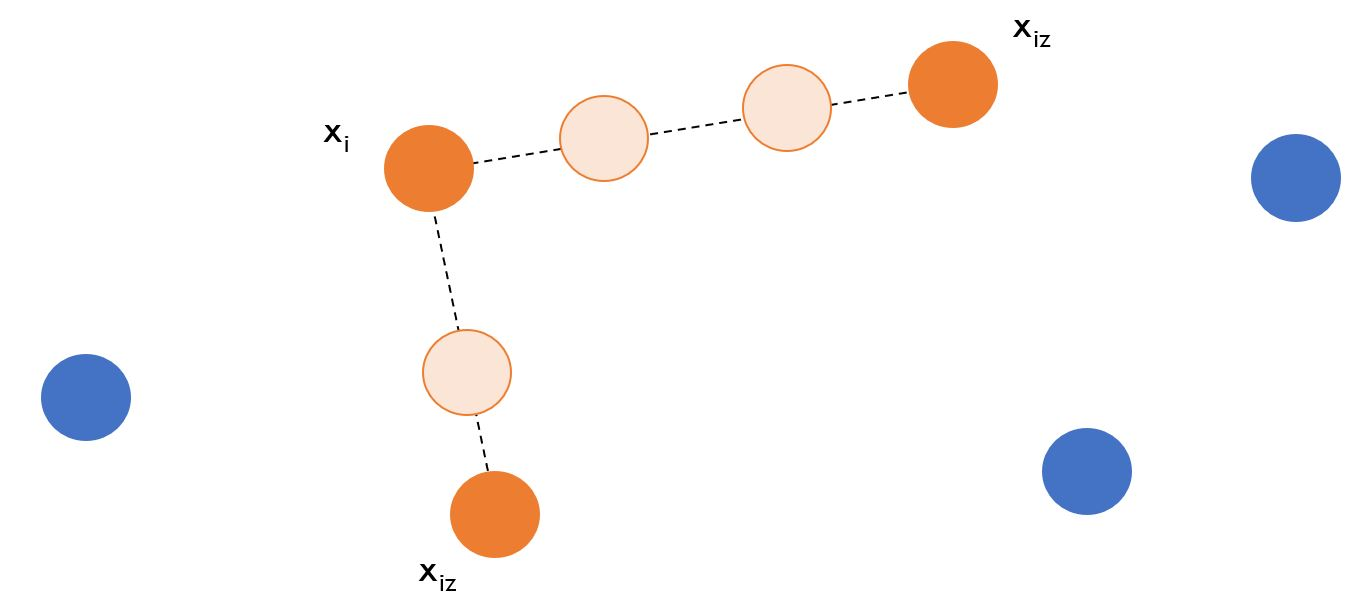
\includegraphics[width=0.9\textwidth]{images/ch3/smote.jpeg}
    \caption{A visual representation of SMOTE.}
    \label{fig:03smote}
\end{figure}

\subsubsection{ADASYN}
The last method is an adaptive version of SMOTE called ADASYN. ADASYN offers "targeted" data generation---more synthetic data is generated for neighbourhoods where the minority class is heavily dominated by the majority class.  For example, suppose the minority class is distributed into two distinct clusters, with one cluster having significantly more minority data compared to the other.  When training a ML model on such a data set, the model will perform significantly better on the minority-dense cluster.  ADASYN can be applied here to target more data generation on the less dense cluster, resulting in comparable model performance for both clusters.  However, ADASYN does not work for sparsely distributed minority classes where only one data point is present.  Additionally, some less dense clusters are a result of noise.  When ADASYN is applied on such clusters, inaccurate minority data will be created which greatly decrease model accuracy during deployment. A more detailed explanation of ADASYN can be found in \cite{adasyn}.


\section{Anomaly Detection and Prediction}
One of the simplest, yet very effective, classification machine learning algorithm is the logistic regression \cite{log_reg}. Logistic regression is a binary \textit{classification} algorithm (although called "regression") that outputs a value between 0 - 1, denoting the probability of a certain event occurring.  For example, the output value to a logistic regression model trained on pump failure data denotes the probability of the pump failing. The model structure of the logistic regression is given as:
\begin{equation}
    \hat{y} = \frac{1}{1 + e^{-(W_1^Tx_1 + W_2^Tx_2 + ... + b)}}
    \label{eq:02LogS}
\end{equation}
where $e$ denotes the exponential operator.  For multi-class classification, softmax functions are typically used and are given by:
\begin{equation}
    y = \frac{e^{z_i}}{\sum\limits^k_{j=0}e^{z_j}}
    \label{eq:03softmax}
\end{equation}
where $z_i$ is given as:
$$z_i = W_{i, 1}^Tx_1 + W_{i, 2}^Tx_2 + ... + b_i$$
The dimensions of the parameter matrices are $W_{j \times k}$ and $b_{j \times 1}$.  Here, $j$ amd $k$ denote the number of classes and the number of features for each data point, respectively.  Lastly, softmax are typically used because the function is continuously differentiable, thus allowing for gradient methods to be viable.

\subsection{Deep Learning Classification and Prediction}
A deep learning binary classification model simply modifies the regression neural network (introduced in the neural networks basic section in Chapter 1) by replacing the last layer's activation function to a sigmoid function. More specifically, the following is the mathematical procedure of the regression neural network model:
\begin{center}
    $z^{[1]}_j = W^{[1]}x + b^{[1]}$ \\
    $a^{[1]}_j = ReLU(z^{[1]}_j)$ \\
    $z^{[2]}_j = W^{[2]}a^{[1]}_j + b^{[2]}$ \\
    $a^{[2]}_j = ReLU(z^{[2]}_j)$ \\
    ... \\
    $z^{[r]}_j = W^{[r]}a^{[r - 1]}_j + b^{[r]}$ \\
    $a^{[r]}_j = ReLU(z^{[r]}_j)$ \\
    $y = W^{[o]}a^{[r]}_j + b^{[o]}$ \\  
\end{center}
In classification, the last step is simply replaced with:
$$z = W^{[o]}a^{[r]}_j + b^{[o]}$$
\begin{equation}
    y = \frac{1}{1 + e^{-z}}
    \label{eq:03sigmoidact}
\end{equation}
For multi-class deep learning classification, the output activation layer is replaced with the softmax function given in Equation \ref{eq:03softmax}.

\subsection{Cost Function for Classification}
The classification models are trained using the following convex cost function:
\begin{equation}
    J = \frac{1}{N}\sum\limits^N_{i=1} y_i \cdot log(f(x_i)) + (1 - y_i) \cdot log(1 - f(x_i))
    \label{eq:03maxentropy}
\end{equation}
where $N$ denotes the total number of training data used for this update step (i.e., the size of the mini-batch).  Here, $y_i$ is the label of the $i^{th}$ training data and $f(x_i)$ is the probability output of the classification model.  Intuitively, the cost function penalizes incorrect misclassifications.  For example, if $y_i = 1$ and $f(x_i) = 1$, then the cost function would be zero.  Likewise, if $y_i = 1$ and $f(x_i) = 0$, the cost function would instead return 1.



\section{Model Performance Assessment}
Often times, accuracy (i.e., \% of times the model predicted accurately) is a poor performance metric for heavily imbalanced data sets.  For example, a model that only predicts false for a classification data set where 99\% of the data is false will still result in a 99\% accuracy even though the model has no predictive capabilities. In such data sets, \textbf{precision} and \textbf{recall} are more proper evaluations of model performance \cite{prec_recall}.

\textbf{Precision:} Percent of time the model successfully predicted a true positive and is given as:
\begin{equation}
    Precision = \frac{TP}{TP + FP}
\end{equation}
where $TP$ and $FP$ denotes the true and false positives, respectively. A model with poor precision results in excessive false alarms and lead to operator complacency quickly.  

\textbf{Recall:} Percent of total events detected, given as:
\begin{equation}
    Recall = \frac{TP}{TP + FP}
\end{equation}
A poor recall model misses many anomalous events.

Typically, there is a trade-off between precision and recall for traditional methods. This could be eliminated, to an extent, using deep learning models trained on a large repository of data \cite{deeplearning_course}.  An acceptable precision and recall depends on the particular application.  For example, highly safety critical systems would require a near perfect recall because even missing one event could lead to catastrophic damage; therefore, a degree of false alarms is acceptable.  On the other hand, safety non-critical applications may favor a high precision model where every alarm should be guaranteed to correspond to an actual event. In non-safety critical applications, false alarms may lead to operator complacency. There do exist models with both high precision and recall; however, such models require vastly more data to identify.



\section{Industrial Product Design}

\subsection{Anomaly Detection}



\subsection{Anomaly Prediction}


\subsection{Interpreting ML Models}
Another critical requirement of ML models is that it must provide \textbf{real value} to the operators.  The algorithms presented here create value in two ways: 1) Provide explainability to the models which can increase intuition and gain addition buy-in from project shareholders and potential users; 2) provide actionable recommendations to operators.  It is almost useless to tell the operators that the plant will blow up in 10 minutes if no details on how to avoid such a fate is not provided.

The model weights can be analyzed to provide explainability for the logistic regression model.

The explainability of neural networks are significantly more difficult compared to logistic regression.  Indeed, even providing a rough explanation is extremely difficult. Some simple approaches include permutation importance, partial dependence plots, and SHAP.  

\textbf{Permutation importance:} Permutation importance identifies the importance of each input feature to the ML model and is applied \textit{after} the model is identified.  In permutation importance, the columns of the features are shuffled, one at a time.  After each shuffle, the model is re-evaluated with  one incorrect feature data.  Here, if the model's performance significantly reduces after the shuffling of a feature, that shuffled feature is deemed to have high predictive power.  On the other hand, if the model performance is unaffected, then the shuffled feature is assumed to have little to no predictive power. This step is repeated for all features in the feature space. More details regarding permutation importance can be found in \cite{perm_imp}, an example of feature shuffling is shown in Figure \ref{fig:03perm_imp}.
\begin{figure}[H]
    \centering
    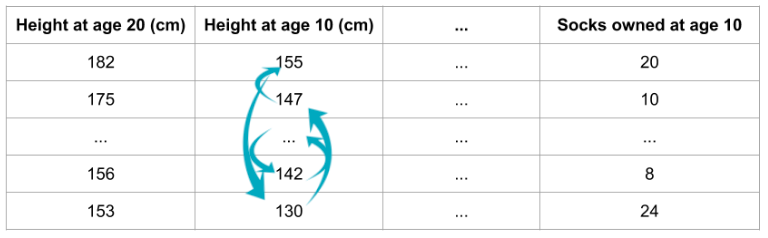
\includegraphics[width=0.8\textwidth]{images/ch3/perm_imp.jpeg}
    \caption{A visual example of permutation importance. Original image from \cite{img_perm_imp}.}
    \label{fig:03perm_imp}
\end{figure}


\textbf{Partial dependence plots:} Partial dependence plots (PDPs) are also evaluated after a model is identified and are used to show how each feature affects the final model prediction.  On a high level, PDPs are similar to evaluating the weights of the models, except PDPs also capture additional, more complex, relationships.  Basically, the fitted model is used to predict for the output while keeping all variables constant except for one.  

Figure \ref{fig:03pdp} shows an example of a PDP plot for one variable.  The y-axis shows the change in the prediction (in this case, winning "Player of the Game" in soccer) while the x-axis is the number of goals scored. Here, the number of goals scored is the variable being manipulated. The plot shows how the chance of winning "Player of the Game" changes as more goals are scored by a player.  In this particular example, the PDP shows that scoring one goal helps tremendously in obtaining player of the game; however, any additional goals provide no impact. For more information on PDPs, see \cite{pdp}.

\begin{figure}[H]
    \centering
    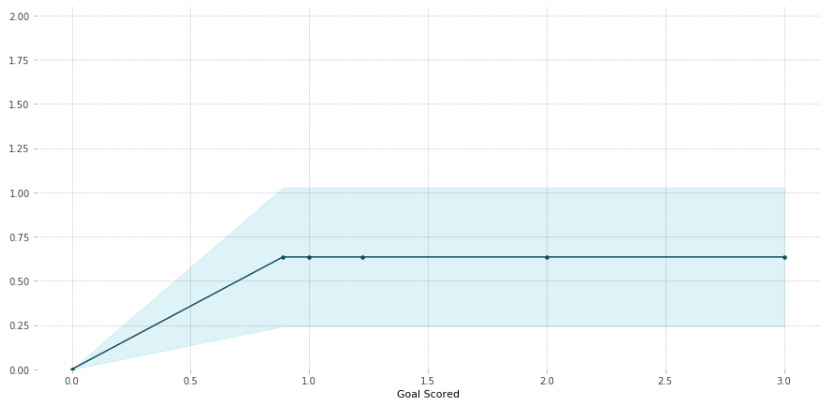
\includegraphics[width=0.8\textwidth]{images/ch3/pdp.jpeg}
    \caption{A visual example of permutation importance. Original image from \cite{pdp_plot}.}
    \label{fig:03pdp}
\end{figure}


\textbf{SHAP:} Shapley additive explanations (SHAP) decomposes model predictions to identify the impact factor of each variable.  This analysis is critical for safety-sensitive systems; by applying SHAP, positive anomaly predictions can be decomposed to identify the root case.


A more detailed description of SHAP can be found in \cite{SHAP}.



\section{Alarm Management}
Industry today is plagued with many problems that require advanced algorithms to overcome. Two of the largest problems are production optimization and alarm management. With continually pressure from environmental groups and increasing government regulations, large industrial companies are forced reduce their environmental footprints while improving the quality of output. The status quo also believes in zero-incident policies, i.e., all workplace incidents are preventable and unacceptable; therefore, it is in the best interest of the companies to implement effective safety systems or their social license to operate could be compromised. To tackle these issues, the University of Alberta's process control team applied artificial intelligence (AI) algorithms in conjunction with classical approaches to an industrial scale wastewater treatment plant (WWTP). The objectives were threefold: i) Design self-learning and adaptive RL controllers to seek out optimal operating strategies. In this case, the controllers must identify the optimal policy to meet government regulations in the most energy efficient way; ii) adaptability feature, allowing the RL controller to learn optimal operating strategies as the operating conditions change, i.e. adapting to changes in season, new government regulations, etc; iii) alarm reduction and prioritization through pattern recognition and communication establishment between RL and the alarm system. Objectives 1 and 2 will be discussed in Chapter 5, objective 3 will be discussed in the following subsections.

Traditionally, alarms were the first line of defense against abnormalities in chemical processes, and were very effective. Due to their cost of implementation, many teams of engineers and subject matter experts would gather together to brain storm the most effective alarm strategies. However, today's plants are littered with alarms due to the price of alarms plummeting after the invention of digital alarms. And because of their sheer number, many alarms are redundant and convey no additional new information.
This project aims to drastically reduce the amount of alarms flooding the alarm console so operators will avoid being overwhelmed. Secondly, this project will prioritize the most important alarms so operators can focus their attention on the highest threats first.

\subsection{Alarm Reduction}

\subsection{Alarm Prioritization}

